\begin{figure}[h]
	\centering
	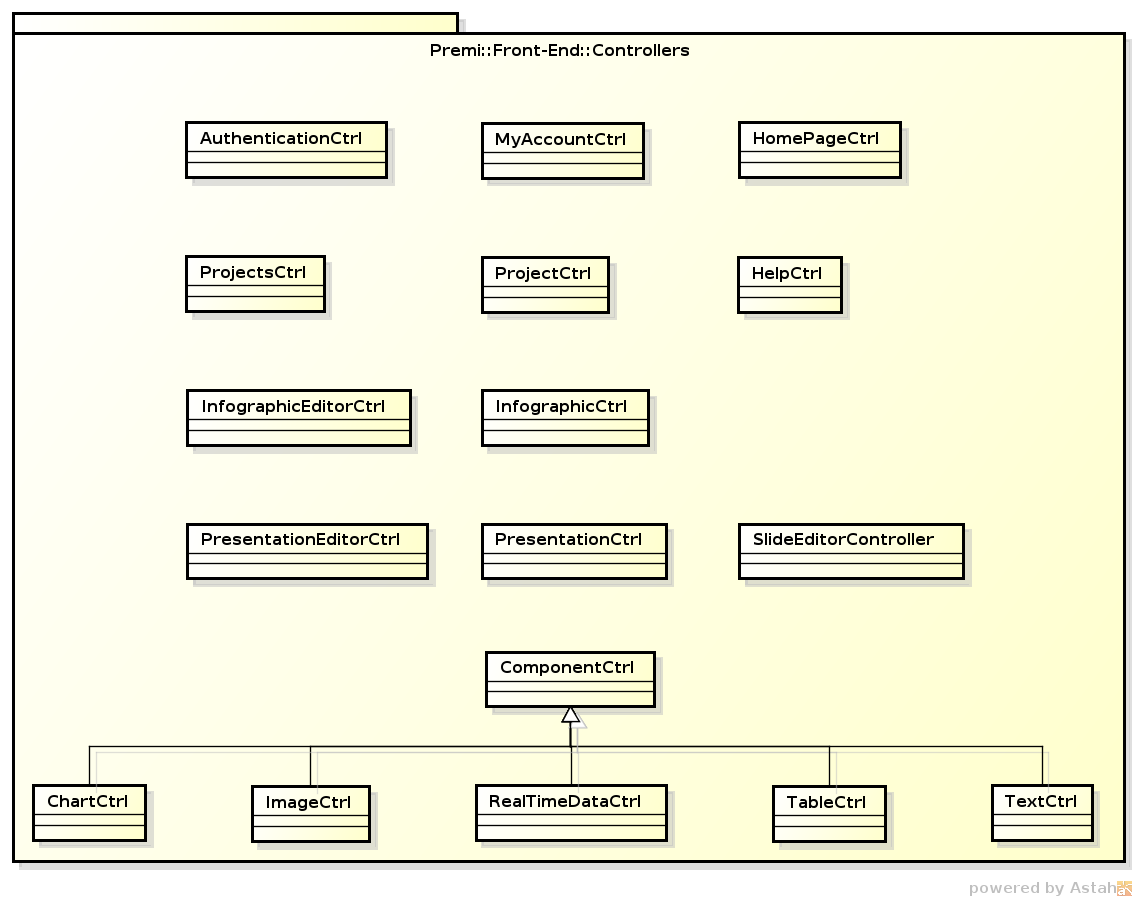
\includegraphics[width=0.7\linewidth]{img/premi_front_end_controllers}
	\caption[Premi::Front-End::Controllers]{Premi::Front-End::Controllers}
\end{figure}
Il package gestisce i controller del front-end dell'applicazione. Comunica con il model, le view e i service della struttura per gestire tutte le operazioni tra di essi. Fa comunicare le view con il model per rendere visibili gli aggiornati effettuati con quest'ultimo e viceversa, aggiorna il model con le informazioni provenienti dalla view. Richiama inoltre i service per comunicare con il back-end e caricare o salvare quindi i dati nel database.
\newpage

\subsubsection{ComponentController}

\subsubsection{HelpController}

\subsubsection{InfographicEditorController}

\subsubsection{LoginController}

\subsubsection{PresentationController}

\subsubsection{PresentationEditorController}
\begin{figure}[h]
	\centering
	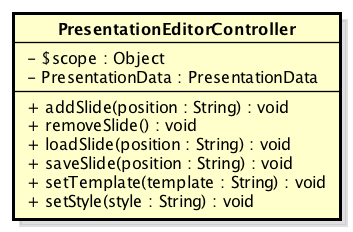
\includegraphics[width=0.5\linewidth]{img/premi_front_end_controllers_presentationeditorcontroller}
	\caption[Premi::Front-End::Controllers::PresentationEditorController]{Premi::Front-End::Controllers::PresentationEditorController}
\end{figure}

	\paragraph{Descrizione}
	Il controller PresentationEditorController si occupa della modifica di una presentazione con i metodi per gestire le slide.
	
	\paragraph{Utilizzo}
	Questa classe viene utilizzata per consentire all'utente di aggiungere o rimuovere una slide dalla presentazione e spostarsi tra di esse. Permette inoltre di impostare lo stile e il template della presentazione.
	
	\paragraph{Attributi}
	\begin{itemize}
		\item \textbf{- PresentationData: PresentationData}:\\
				Campo dati che contiene un riferimento al servizio che si occupa della gestione dei dati e delle impostazioni di una presentazione;
		\item \textbf{\$scope: Object}:\\
				Campo dati contenente un riferimento all'oggetto \$scope creato da Angular, viene utilizzato come mezzo di comunicazione tra il controller e la view. Contiene gli oggetti che definiscono il model dell'applicazione.
	\end{itemize}
	
	\paragraph{Metodi}
	\begin{itemize}
		\item \textbf{addSlide(position: String)}:\\
				Metodo che aggiunge una slide alla presentazione rispetto alla slide corrente nella posizione indicata da \textit{position};
		\item \textbf{removeSlide()}:\\
				Metodo che rimuove la slide corrente dalla presentazione;
		\item \textbf{loadSlide(position: String)}\\
				Metodo che carica la slide nella posizione indicata da \textit{position};
		\item \textbf{saveSlide(position: String)}\\
				Metodo che salva la slide della posizione indicata da \textit{position};
		\item \textbf{setTemplate(template: template)}
				Metodo che imposta il template per la presentazione con quello passato per parametro;
		\item \textbf{setStyle(style: style)}
				Metodo che imposta lo stile della presentazione con quello passato per parametro.
	\end{itemize}